\section{Introduction}
\label{sec:introduction}

Surface electromyography (sEMG) pattern recognition provides a practical interface for multifunction myoelectric control \citep{hudgins1993new,englehart2003robust,scheme2011electromyogram,farina2014extraction}, but its performance depends partly on the number and spatial distribution of recording sites. Increasing the number of electrodes can provide richer spatial information, yet each additional electrode also increases hardware complexity, wiring, skin-contact area, setup requirements and potential points of failure \citep{vujaklija2016new}. Electrode reduction \chg{is therefore} an important design problem: the objective is not simply to remove as many electrodes as possible, but to identify the smallest configuration that preserves an acceptable level of recognition performance.

A substantial literature has addressed channel and feature reduction in sEMG using feature-ranking methods, wrapper approaches, sparse representations, and multi-channel or high-density electrode arrays \citep{phinyomark2012feature,liu2014emg,altimemy2013classification,stango2015spatial,qu2021reduce}. However, three methodological issues complicate the translation of these results to devices intended for use across individuals.

First, electrode subsets are frequently selected and evaluated within the same users. Such user-dependent designs are appropriate for personalised systems, but they do not establish whether a common reduction strategy will generalise to an unseen user. Subject-independent recognition poses a more stringent problem because inter-individual anatomical and physiological variability can alter both the recorded signals and the spatial distribution of discriminative information \citep{phinyomark2018emg,cote2019deep}. Moreover, allowing information from the eventual test participant to influence standardisation, ranking or model selection introduces optimistic bias.

Second, model-attribution methods provide an appealing means of identifying informative recording sites but introduce their own methodological challenges. TreeSHAP, for example, estimates the contribution of \chg{each model input to a prediction} \citep{lundberg2017unified,lundberg2020local}\chg{; these contributions can be aggregated} to rank electrodes, as has been done for channel reduction in other biosignal tasks \citep{salmi2025shapaad}. Yet attribution estimates may vary across training samples \citep{visani2022statistical,kelodjou2023shaping}, and a ranking derived from the same data used for evaluation can itself become a source of information leakage. A valid subject-independent electrode-selection procedure must therefore estimate electrode importance without allowing the test participant to influence either the attributing model or the resulting ranking. Treating attributions as distributions across resamples and penalising \chg{features whose attributions are unstable} has also been proposed \citep{xiang2026roshap,meinshausen2010stability}; the stability penalty tested here is related to that idea and is not claimed as new.

Third, determining the number of electrodes to retain is often treated descriptively: an accuracy curve is inspected and a visually acceptable operating point is selected. Such an approach does not formally define how much performance loss is acceptable \citep{schuirmann1987comparison,walker2011understanding}. If the tolerance is chosen after observing the reduction curve, the resulting claim cannot be interpreted as a prespecified non-inferiority decision \citep{campbell2018noninferiority}. A more defensible formulation is therefore to define the acceptable loss in advance and evaluate reduced configurations against that threshold.

The present study addresses these issues through a participant-level, cross-fitted evaluation framework (figure~\ref{fig:overview}). For each outer leave-one-subject-out fold, the held-out participant is excluded from feature standardisation, model fitting and electrode ranking. TreeSHAP attributions are estimated on participant-disjoint inner folds, so each attribution is obtained from observations not used to train the corresponding attributing model. Reduced models are subsequently retrained using only the selected electrodes and evaluated on the outer held-out participant. The primary decision rule was specified before the reduced-array performance curve was examined: a subset was considered non-inferior when the lower bound of the participant-level confidence interval for its Macro-F1 difference from the full array \chg{exceeded $-0.02$, that is, a non-inferiority margin of 0.02 Macro-F1.}

Rather than introducing attribution as a new selection algorithm, the study evaluates whether attribution-guided selection provides useful and reproducible information under a leakage-controlled, subject-independent design, using the 43-participant GRABMyo dataset \citep{pradhan2022multiday}. The analysis plan posed four study questions. The primary question (H1), whose non-inferiority decision rule was fixed in advance, is whether any reduced subset is non-inferior to the complete 16-electrode array. The secondary questions are (H2) whether attribution-ranked subsets outperform random subsets of the same size, (H3) whether penalising attribution instability improves selection relative to attribution magnitude alone, and (H4) whether the ranking is faithful, that is, whether removing highly ranked electrodes and retraining degrades performance more than removing weakly ranked ones; the detailed test families for H2--H4 were specified later. Because every ranking is recomputed within each outer fold, the design evaluates a reduction procedure and the electrode count it supports, rather than one fixed physical layout. Additional exploratory analyses examine ranking stability across participants, transfer across recording sessions, bipolar re-referencing, replication on NinaPro DB5 \citep{pizzolato2017comparison}, and participant-level aggregation of attribution variability. Both positive and null findings are reported.

\begin{figure}[t]
\centering
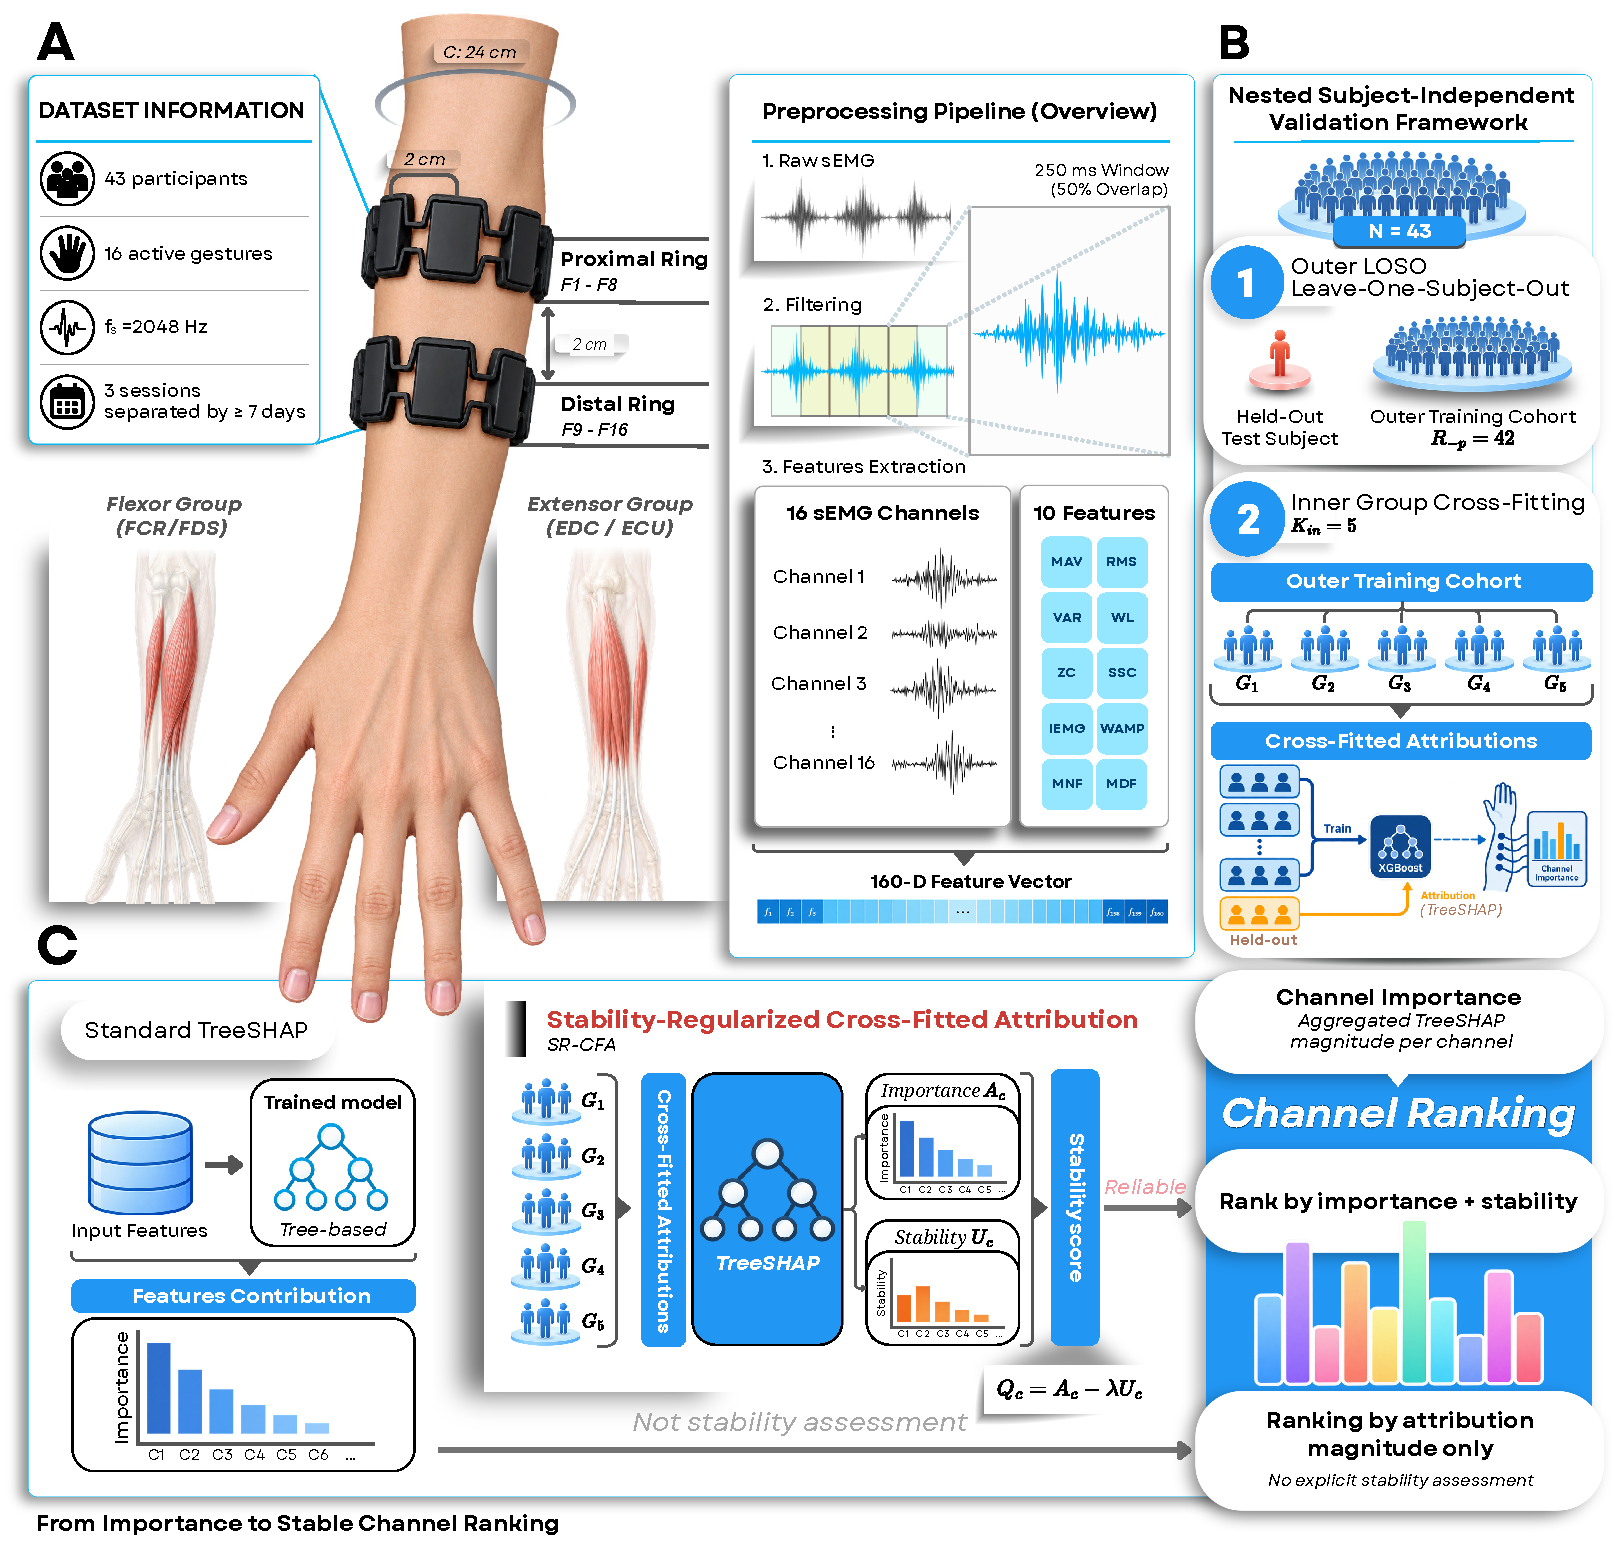
\includegraphics[width=\textwidth]{figures/fig1_overview.pdf}
\caption{Study overview. (A) GRABMyo data and preprocessing: two circumferential rings of eight monopolar electrodes 2~cm apart on the forearm (proximal ring F1--F8, distal ring F9--F16), 250~ms analysis windows with 50\% overlap and ten features per channel (160 features per window). Electrode housings are drawn schematically, and the muscle drawings show general forearm anatomy only; electrodes were not registered to individual muscles. (B) Subject-independent validation: each participant is held out in turn (outer leave-one-subject-out split), and attributions are computed by cross-fitting over five participant-disjoint groups of the remaining participants. (C) The two electrode rankings compared in this study: cross-fitted attribution magnitude alone ($\lambda = 0$) and the stability-regularised score $Q_c = A_c - \lambda U_c$ (SR-CFA). The panel shows how the rankings are formed, not which performed better; the stability penalty produced no statistically detectable improvement (section~\ref{sec:res_attribution}).}
\label{fig:overview}
\end{figure}
